\chapter{Preparation}
\section{Loss Mechanisms in Optical Fibers}

\subsection{Principles of Wave Guiding in Optical FIbers}
The guiding mechanism of a mode in an optical fiber can be described by an electromagnetic wave model. A wave hitting a dielectic boundary at a certain angle is reflected completely. For a waveguide structure like shown in figure \ref{fig:slab1} the wave is confined to the core, when the incident angle $\theta$ is smaller than the angle of total reflection. But since the Fields in the waveguide propagate as waves an additional condition has to be fulfilled. The x component of the Fields has to be a standing wave, because else it would deplete itself. Thus the wavenumber in the core in x direction times the height of the core $k\i{1x}h$ plus the phase jump caused by the reflections on the boundarys has to be an integer multiple of $\pi$:
\begin{equation}
 -2k\i{1x}h+2\varphi = -m\cdot2\pi
\end{equation}
This leads to several guided modes in a waveguide structure, dependent on the height of the core and the used materials. The described principle can be easyly transferred to cylindrically symetric structures like fibers or even more complex geometries.

\subsection{Loss Mechanisms in Optical Fibers}
\label{loss}
The losses in optical fibers can be explained by different mechanisms. First there is the intrinsic material absorption. From the Kramers-Kronig relation of the real and imaginary part of the dielectric susceptibility it can be derived, that, if the attenuation of a medium is zero ($\chi\i{i}=0$ the medium is also dispersionless ($\chi=0$). Thus every dispersive medium has absorption. Furthermore there are the extrinsic losses in the fiber. These are caused by material impurities in the material like metal or OH$^-$ ions. Another source of losses is the Rayleigh scattering. This scattering is caused by random index fluctuations smaller than a wavelength. These index fluctuations arise during the freezing of the silica molecules during the fiber fabrication. 

\subsection{Bends in Optical Fibers}

When a waveguide is bent it shows significant loss due to radiation. A wavefront propagates with its group velocity. If the waveguide is bent the wavefront at the inner boundary travels further in the same time than the wavefront at the outer boundary. This leads to a bigger part of the field that is not confined to the waveguide core. If the waveguide is bent further the fiber can break.


\section{Optical Time Domain Reflectometry}
Optical time domain reflectometry (OTDR) is a methodology to measure and characterize optical networks. It is possible to estimate losses in the fiber caused by connections or damages of the fiber. The attenuation of the fiber can be estimated just as the fiber length.

\subsection{Measurement principles of OTDR}
To analyze an optical network wit OTDR an optical time domain reflectometer sends in a short laser pulse with a certain amount of energy. The pulse travels trough the fiber and gets reflected and scattered at fiber connections, switches, damages and impurities in the fiber. 

After sending the pulse into the fiber the reflectometer starts listening on the port. An directional coupler leads the incoming light to a photodetector. Using the photodetector backscattered light can be detected. The time when the backscattered signal comes in is used to calculated the distance of the location the light got scattered.
There are two kinds of reflections that are important for the OTDR.
The Fresnel reflection is caused by an index contrast. This is the case at a splice, an open connection or a damaged fiber. Figure \ref{fig:fresnel}\footnotemark[1] shows different Fresnel reflections that can be measured. Empirical knowledge of the reflections of different connection and events gives information about the detected reflection.
 

\begin{figure}%
\centering
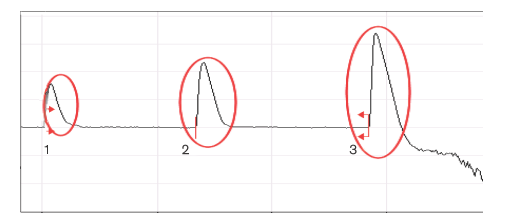
\includegraphics[width=.6\columnwidth]{Grafiken/fresnel.png}%
\caption{Different Fresnel reflection caused by by (1) mechanical splices, (2) bulkhead and (3) open connection}%
\label{fig:fresnel}%
\end{figure}

The other scattering mechanism is the Rayleigh scattering (cf. \ref{loss}). The result of Rayleigh scattering is a straight slope in the OTDR trace. With that information the attenuation of the fiber can be calculated.\footnote[1]{EXFO - Application Note 194}





\


\section{Characterisation of Passive Optical Networks}